\documentclass[11pt,a4paper,twoside]{jarticle}
%==== 科研費LaTeX =============================================
%	2013(H25)年度 基盤研究(A,B)(一般)
%============================================================
% 2007-08-19: Taku Yamanaka (JSPS Research Center for Science Systems / Osaka Univ.)
%		Switched to kakenhi3.sty.
% 2007-09-18: Taku: Do not show the budget table beyond the final year.
%============================================================
%=======================================
% form00_header.tex
%	General header for kakenhiLaTeX,  Moved over from form00_2010_header.tex.
%	2009-09-06 Taku Yamanaka (Osaka Univ.)
%==== General Version History ======================================
% 2006-05-30 Taku Yamanaka (Physics Dept., Osaka Univ.)
% 2006-06-02 V1.0
% 2006-06-14 V1.1 Use automatic calculation for cost tables.
% 2006-06-18 V1.2 Split user's contents and the format.
% 2006-06-20 V1.3 Reorganized user and format files
% 2006-06-25 V1.4 Readjusted all the table column widths with p{...}.
%				With \KLTabR and \KLTabRNum, now the items can be right-justified
%				in the cell defined by p{...}.
% 2006-06-26 V1.5 Use \newlength and \setlength, instead of \newcommand, to define positions.
% 2006-08-19 V1.6 Remade it for 2007 JFY version.
% 2006-09-05 V1.7 Added font declarations suggested by Hoshino@Meisei Univ.
% 2006-09-06 V1.8 Introduced usePDFform flag to switch the form file format.
% 2006-09-09 V1.9 Changed p.7, to allow different heights between years. (Thanks to Ytow.)
% 2006-09-11 V2.0 Added an option to show budget summary.
% 2006-09-13 V2.1 Added an option to show the group.
% 2006-09-14 V2.1.1 Cleaned up Kenkyush Chosho.
% 2006-09-21 V2.2 Generated under a new automatic development system.

% 2007-03-24 V3.0 Switched to a method using "picture" environment.

% 2007-08-14 V3.1 Switched to kakenhi3.sty.
% 2007-09-17 V3.2 Added \KLMaxYearCount
% 2008-03-08 V3.3 Remade it for 2009 JFY version\
% 2008-09-08 V3.4 Added \KLXf ... \KLXh.
% 2011-10-20 V5.0 Use kakenhi5.sty, to utilize array package in tabular environment.
% 2012-08-14 v5.1 Moved preamble and kakenhi5 into the current directory, instead of the parent directory.
%=======================================
%============================================================
% preamble.tex
%
% Dummy section and subsection commands.
% With these, some editors (such as TeXShop, etc.) can jump to the (sub)sections.
\newcommand{\dummy}{dummy}% 
\renewcommand{\section}[1]{\renewcommand{\dummy}{#1}}
\renewcommand{\subsection}[1]{\renewcommand{\dummy}{#1}}

% Flag for switching form file format.......
\usepackage{ifthen}
\newboolean{usePDFform}
\newboolean{BudgetSummary}

\usepackage{forms/kakenhi5}

\pagestyle{empty}

% ===== Parameters for LaTeX =========================

% ===== Font declarations  ======================================
\DeclareFontShape{JT1}{mc}{m}{it}{<->ssub * mc/m/n}{}
\DeclareFontShape{JY1}{mc}{m}{it}{<->ssub * mc/m/n}{}

% ===== Parameters for KL (Kakenhi LaTeX) ========================
% general purpose temporary variables	-2007
\newcommand{\KLX}{}
\newcommand{\KLXa}{}
\newcommand{\KLXb}{}
\newcommand{\KLXc}{}
\newcommand{\KLXd}{}
\newcommand{\KLXe}{}
\newcommand{\KLXf}{}
\newcommand{\KLXg}{}
\newcommand{\KLXh}{}
\newcommand{\KLY}{}
\newcommand{\KLYa}{}
\newcommand{\KLYb}{}
\newcommand{\KLXR}{}
\newlength{\KLCella}
\newlength{\KLCellb}
\newlength{\KLCellc}
\newlength{\KLCelld}
\newlength{\KLCelle}
\newlength{\KLCellf}
\newlength{\KLCellg}
\newlength{\KLCellh}

% sub-page
\newlength{\KLSubPageX}
\newlength{\KLSubPageY}
\newlength{\KLspx}
\newlength{\KLspy}
\newcommand{\KLSubPageXmm}{}	% for \input(x,y){....} which uses a unit (mm)
\newcommand{\KLSubPageYmm}{}	% for \input(x,y){....} which uses a unit (mm)

% margins for parbox inside frames; in units of points
\newcounter{KLParboxSideMargin}
\newcounter{KLParboxTopMargin}
\newcounter{KLParboxBottomMargin}

% ===== standard counters ======================================
\newcounter{KLSubPageNo}	% sub-page counter
\newcounter{KLPageOffset}		% to generate sub-page number
\newcounter{KLMaxYearCount}	% # of years for the proposal


% ===== initializations ============
\KLInitTypesettingPageSelection



% user01_header
%=== 様式のファイルの形式の指定 =====================
%   epsではなく、PDF の様式を読み込む場合は、次の行の頭の%を消してください。
%\setboolean{usePDFform}{true}
%=======================================

%=== 予算の表の印刷 =====================
% 予算の集計の表を出すためには、次の行の頭の%を消してください。
%\setboolean{BudgetSummary}{true}
%=================================

% === 一部のページだけタイプセット ==============
% New in 2009 fall version!
% 選んだページだけタイプセットするには、次の例の頭の%を消し、並べてください。
% 複数のページを選ぶこともできます。
% 提出前には、必ず全てコメントアウト(頭に%をつける)してください。
%ーーーーーーーーーーーーーーーーーーーーーーーーーーーーーーーーー
%\KLTypesetPage{1}			% p.1 (or p.1を含む連続したページ),
%\KLTypesetPage{3}			% p.3 (or p.3を含む連続したページ),
%\KLTypesetPagesInRange{5}{6}	% p.5 ~ p.6,
%\KLTypesetPagesInRange{8}{10}	% and p.8 ~ p.10
%=================================

% ===== my favorite packages ====================================
% ここに、自分の使いたいパッケージを宣言して下さい。
\usepackage{wrapfig}
% \usepackage{amssymb}
%\usepackage{mb}
%\DeclareGraphicsRule{.tif}{png}{.png}{`convert #1 `dirname #1`/`basename #1 .tif`.png}
%==========================================================

\newcommand{\KLShouKeiLine}[1]{\cline{#1}}
%もし、小計の上の線を取れと事務に言われたら、
%「そのようなことは、記入要項に書かれていないし、学振はそのようなことは気にしていない。」と
% 突っぱねる。
% それでもなお消せと理不尽なことを言われたら、次の行の 最初の「%」を消す。	
%\renewcommand{\KLShouKeiLine}[1]{}

\newcommand{\KLBudgetTableFontSize}{small}	% 予算の表のフォントの大きさ: small, footnotesize

% ===== my personal definitions ==================================
% ここに、自分のよく使う記号などを定義して下さい。
\newcommand{\klpionn}{K_L \to \pi^0 \nu \overline{\nu}}
\newcommand{\kppipnn}{K^+ \to \pi^+ \nu \overline{\nu}}


% hook3: after including packages ===================
 % for future maintenance
% ===== Global definitions for the Kakenhi form ======================
% 基本情報
%
%------ 研究種別 ----------------------------------------------
\newcommand{\研究種別}{A}	% A or B or C

%------ 研究課題名  -------------------------------------------
\newcommand{\研究課題名}{コ・クリエイティブなソフトウェア開発者を育成するPBL型教育}

%----- 研究機関名と研究代表者の氏名-----------------------
\newcommand{\研究機関名}{産業技術大学院大学}
\newcommand{\研究代表者氏名}{中鉢 欣秀}
\newcommand{\研究代表者氏名ふりがな}{ちゅうばち よしひで}
\newcommand{\me}{\underline{\underline{中鉢 欣秀}}}
\newcommand{\meen}{\underline{\underline{Y.~Chubachi}}}

%---- 本研究への研究代表者のエフォート(%)
\newcommand{\本応募effort}{\KLEffort{18}}	% 半角数字のみ

%---- 研究期間の最終年度 ----------------
\newcommand{\研究期間の最終元号年度}{27}	%平成で、半角数字のみ
%=========================================================

% ===== Global year-dependent definitions for the Kakenhi form ===========
% 基本情報
\newcommand{\研究開始年度}{2013}
\newcommand{\研究開始元号年度}{25}	%平成

\newcommand{\1年目西暦}{2013}
\newcommand{\2年目西暦}{2014}
\newcommand{\3年目西暦}{2015}
\newcommand{\4年目西暦}{2016}
\newcommand{\5年目西暦}{2017}
\newcommand{\6年目西暦}{2018}

\newcommand{\1年目}{25}
\newcommand{\2年目}{26}
\newcommand{\3年目}{27}
\newcommand{\4年目}{28}
\newcommand{\5年目}{29}
\newcommand{\6年目}{30}

\newcommand{\1年目J}{25}
\newcommand{\2年目J}{26}
\newcommand{\3年目J}{27}
\newcommand{\4年目J}{28}
\newcommand{\5年目J}{29}
\newcommand{\6年目J}{30}


	% <<< New year ?
%==========================================================
% form03_header.tex
%	2009-03-04: Taku Yamanaka (Osaka Univ.)
%==========================================================
\usepackage{calc}
\usepackage{watermark}
\usepackage{longtable}
\usepackage{geometry}                % See geometry.pdf to learn the layout options. There are lots.
\usepackage{udline}
\usepackage{array}

\geometry{noheadfoot,scale=1}  %scale=1 resets margins to 0
\setlength{\unitlength}{1pt}

% define variables for positions ==========================
% picture environment location, in  units of points
\newcommand{\KLOddPictureX}{}
\newcommand{\KLEvenPictureX}{}
\newcommand{\KLPictureY}{}
\newcommand{\KLOddPictureInWaterMarkX}{}
\newcommand{\KLEvenPictureInWaterMarkX}{}
\newcommand{\KLPictureInWaterMarkY}{}

\newlength{\KLoddsidemargin}
\newlength{\KLevensidemargin}
\newlength{\KLtopmargin}

\newcounter{KLCOddPictureInWaterMarkX}
\newcounter{KLCEvenPictureInWaterMarkX}
\newcounter{KLCPictureInWaterMarkY}
\newcounter{KLCOddPictureX}
\newcounter{KLCEvenPictureX}
\newcounter{KLCPictureY}

%------------------------------------------------------------

\newcommand{\KLLeftEdge}{}
\newcommand{\KLRightEdge}{}

% standard margins for text in frames
\setcounter{KLParboxSideMargin}{7}
\setcounter{KLParboxTopMargin}{12}
\setcounter{KLParboxBottomMargin}{5}


%=================================================================
% form05_kiban_ab_header.tex
%	for the 2007(H19) Japanese Fiscal Year
%	2006-10-01 : Taku Yamanaka (Osaka Univ.)
%			Switched to the new development system using a "mother file".
%	2007-08-08: Taku
%			Switched to a new method using "picture" environment.
%	2007-09-01: Taku
%			Readjusted parameters for the new 2008 form.
%	2009-09-04: Taku
%			Introduced form03_header and form07_header to automatically calculate margins and
%			other miscellaneous coordinate parameters.
%=================================================================

% ===== Global definitions for the Kakenhi form ======================
% 基本情報
\newcommand{\研究種目}{基盤研究}
\newcommand{\研究種目後半}{(一般)}
\ifthenelse{\isundefined{\研究種別}}{
	\newcommand{\研究種別}{}
}{}%
\newcommand{\KLMainFile}{kiban\_ab.tex}
\newcommand{\KLForms}{kiban_ab_forms}
\newcommand{\KLYoshiki}{kiban_ab}

% 奇数ページの下に記入される情報
\newcommand{\klbyYup}{}
\newcommand{\klbyYdown}{}
\newcommand{\klbyKikanXleft}{}
\newcommand{\klbyKikanXright}{}
\newcommand{\klbyNameXleft}{}
\newcommand{\klbyNameXright}{}

\newcommand{\KLBottomInfo}[6]{%
	\ifthenelse{\equal{#1}{}}{%
		\renewcommand{\klbyYup}{69}
		\renewcommand{\klbyYdown}{55}
	}{%
		\renewcommand{\klbyYup}{#1}
		\renewcommand{\klbyYdown}{#2}
	}
	
	\ifthenelse{\equal{#3}{}}{%
		\renewcommand{\klbyKikanXleft}{134}
		\renewcommand{\klbyKikanXright}{349}
		\renewcommand{\klbyNameXleft}{439}
		\renewcommand{\klbyNameXright}{552}
	}{%
		\renewcommand{\klbyKikanXleft}{#3}
		\renewcommand{\klbyKikanXright}{#4}
		\renewcommand{\klbyNameXleft}{#5}
		\renewcommand{\klbyNameXright}{#6}
	}
	\KLTextBox{\klbyKikanXleft}{\klbyYup}{\klbyKikanXright}{\klbyYdown}{}{\研究機関名}%
	\KLTextBox{\klbyNameXleft}{\klbyYup}{\klbyNameXright}{\klbyYdown}{}{\研究代表者氏名}%
}

%==========================================================
% frame edge positions of multi-page-block
\newcommand{\KLOddMultiPageLeftEdge}{65}
\newcommand{\KLOddMultiPageRightEdge}{552}
\newcommand{\KLEvenMultiPageLeftEdge}{43}
\newcommand{\KLEvenMultiPageRightEdge}{530}

% vertical limits in the first multi-page-block
\newcommand{\KLMultiPageTopEdge}{745}		%lowest top position (except for the 1st page)
\newcommand{\KLMultiPageBottomEdge}{70}	%highest bottom position (except for the last page)

% Modify the edges for single page frames if necessary
\newcommand{\KLOddLeftEdge}{\KLOddMultiPageLeftEdge}
\newcommand{\KLOddRightEdge}{\KLOddMultiPageRightEdge}
\newcommand{\KLEvenLeftEdge}{\KLEvenMultiPageLeftEdge}
\newcommand{\KLEvenRightEdge}{\KLEvenMultiPageRightEdge}

%==========================================================

%==========================================================
% form07_header.tex
%	2009-03-04: Taku Yamanaka (Osaka Univ.)
%==========================================================
% Remember Standard Positions that were set in form05_xxxx_header.tex
\let \KLStandardOddMultiPageLeftEdge = \KLOddMultiPageLeftEdge
\let \KLStandardOddMultiPageRightEdge = \KLOddMultiPageRightEdge
\let \KLStandardEvenMultiPageLeftEdge = \KLEvenMultiPageLeftEdge
\let \KLStandardEvenMultiPageRightEdge = \KLEvenMultiPageRightEdge

\let \KLStandardMultiPageTopEdge = \KLMultiPageTopEdge
\let \KLStandardMultiPageBottomEdge = \KLMultiPageBottomEdge

\let \KLStandardOddLeftEdge = \KLOddLeftEdge
\let \KLStandardOddRightEdge = \KLOddRightEdge
\let \KLStandardEvenLeftEdge = \KLEvenLeftEdge
\let \KLStandardEvenRightEdge = \KLEvenRightEdge


% ===== File format for forms ===========================
\ifthenelse{\boolean{usePDFform}}{
	\newcommand{\KLFormFormat}{pdf}	\usepackage[dvipdfm]{graphicx}
}{	\newcommand{\KLFormFormat}{eps}	\usepackage{graphicx}
}

%------ This should be set before \begin{document} ------
\KLStandardLengths
\KLStandardPositions
%----------------------------------------------------------------------------


%============================================================
%endPrelude

\begin{document}
% hook5 : right after \begin{document} ==============
 % for future maintenance
%============================================================
%     User Inputs
%============================================================

%form: kiban_ab_form_01-02.tex ; user: kiban_ab_01-02_purpose.tex
%========== S-1-7 基盤研究(A,B)(一般) =========
%===== p. 01-02 研究目的 =============
\section{研究目的}
%watermark: w02_purpose_AB
\newcommand{\研究目的概要}{%
%begin  研究目的概要===================
	コ・クリエイティブなソフトウェア開発方法論とは,ソフトウェア開発者がマーケットとの直接的な対話を通して
	市場でマネタイズできるソフトウェアサービスを開発するための新しい開発プロセスである.本研究では,この
	開発プロセスをプロジェクト型学習(PBL)により教育するための教材および教授法を開発することを目的とする.
	
	本研究者らが行なってきたPBLによるソフトウェア技術者の教育実績を踏まえ,指導者のためのガイドライン,
	PBLを支援するためのインフラストラクチャー,その他必要な教材の整備を行い,この教育手法を確立させ,
	次世代型のソフトウェア開発者育成法として普及を図る.
%end  研究目的概要 ====================
}

\newcommand{\研究目的}{%
%begin  研究目的===================
	
	\begin{flushleft}
		■コ・クリエイティブなソフトウェア開発
	\end{flushleft}

    「コ・クリエイション(co-creation)」とは,マーケティング分野の用語であり,
    商品やサービスの開発にあたり企業が顧客を巻き込むことでよりよいものを創りだすことを指す.
    コ・クリエイションの最近の事例としては,Starbucks,Dellなどが顧客のアイディア
    をソーシャルメディアにより収集し,自社のサービス改善につなげていることが報告されている\cite{wired}.

    一方で,ソフトウェア開発においては,従来からLinuxを代表とするオープンソース型の
    ソフトウェア開発のスタイルに見られるように,コ・クリエイティブにソフトウェアプロダクトを開発する事例が数多くある.
    ソフトウェアを開発するデベロッパーとユーザとの間に垣根がなく,ユーザは自ら必要とする機能を追加することさえできる.
    これにより,開発者と利用者が共になって新しいソフトウェアを創造することを通して,価値のあるプロダクトが生まれてきた.
	
	\begin{flushleft}
		■IT産業界の現状
	\end{flushleft}
    
         \begin{wrapfigure}{r}{7cm}
         		\begin{center}
		         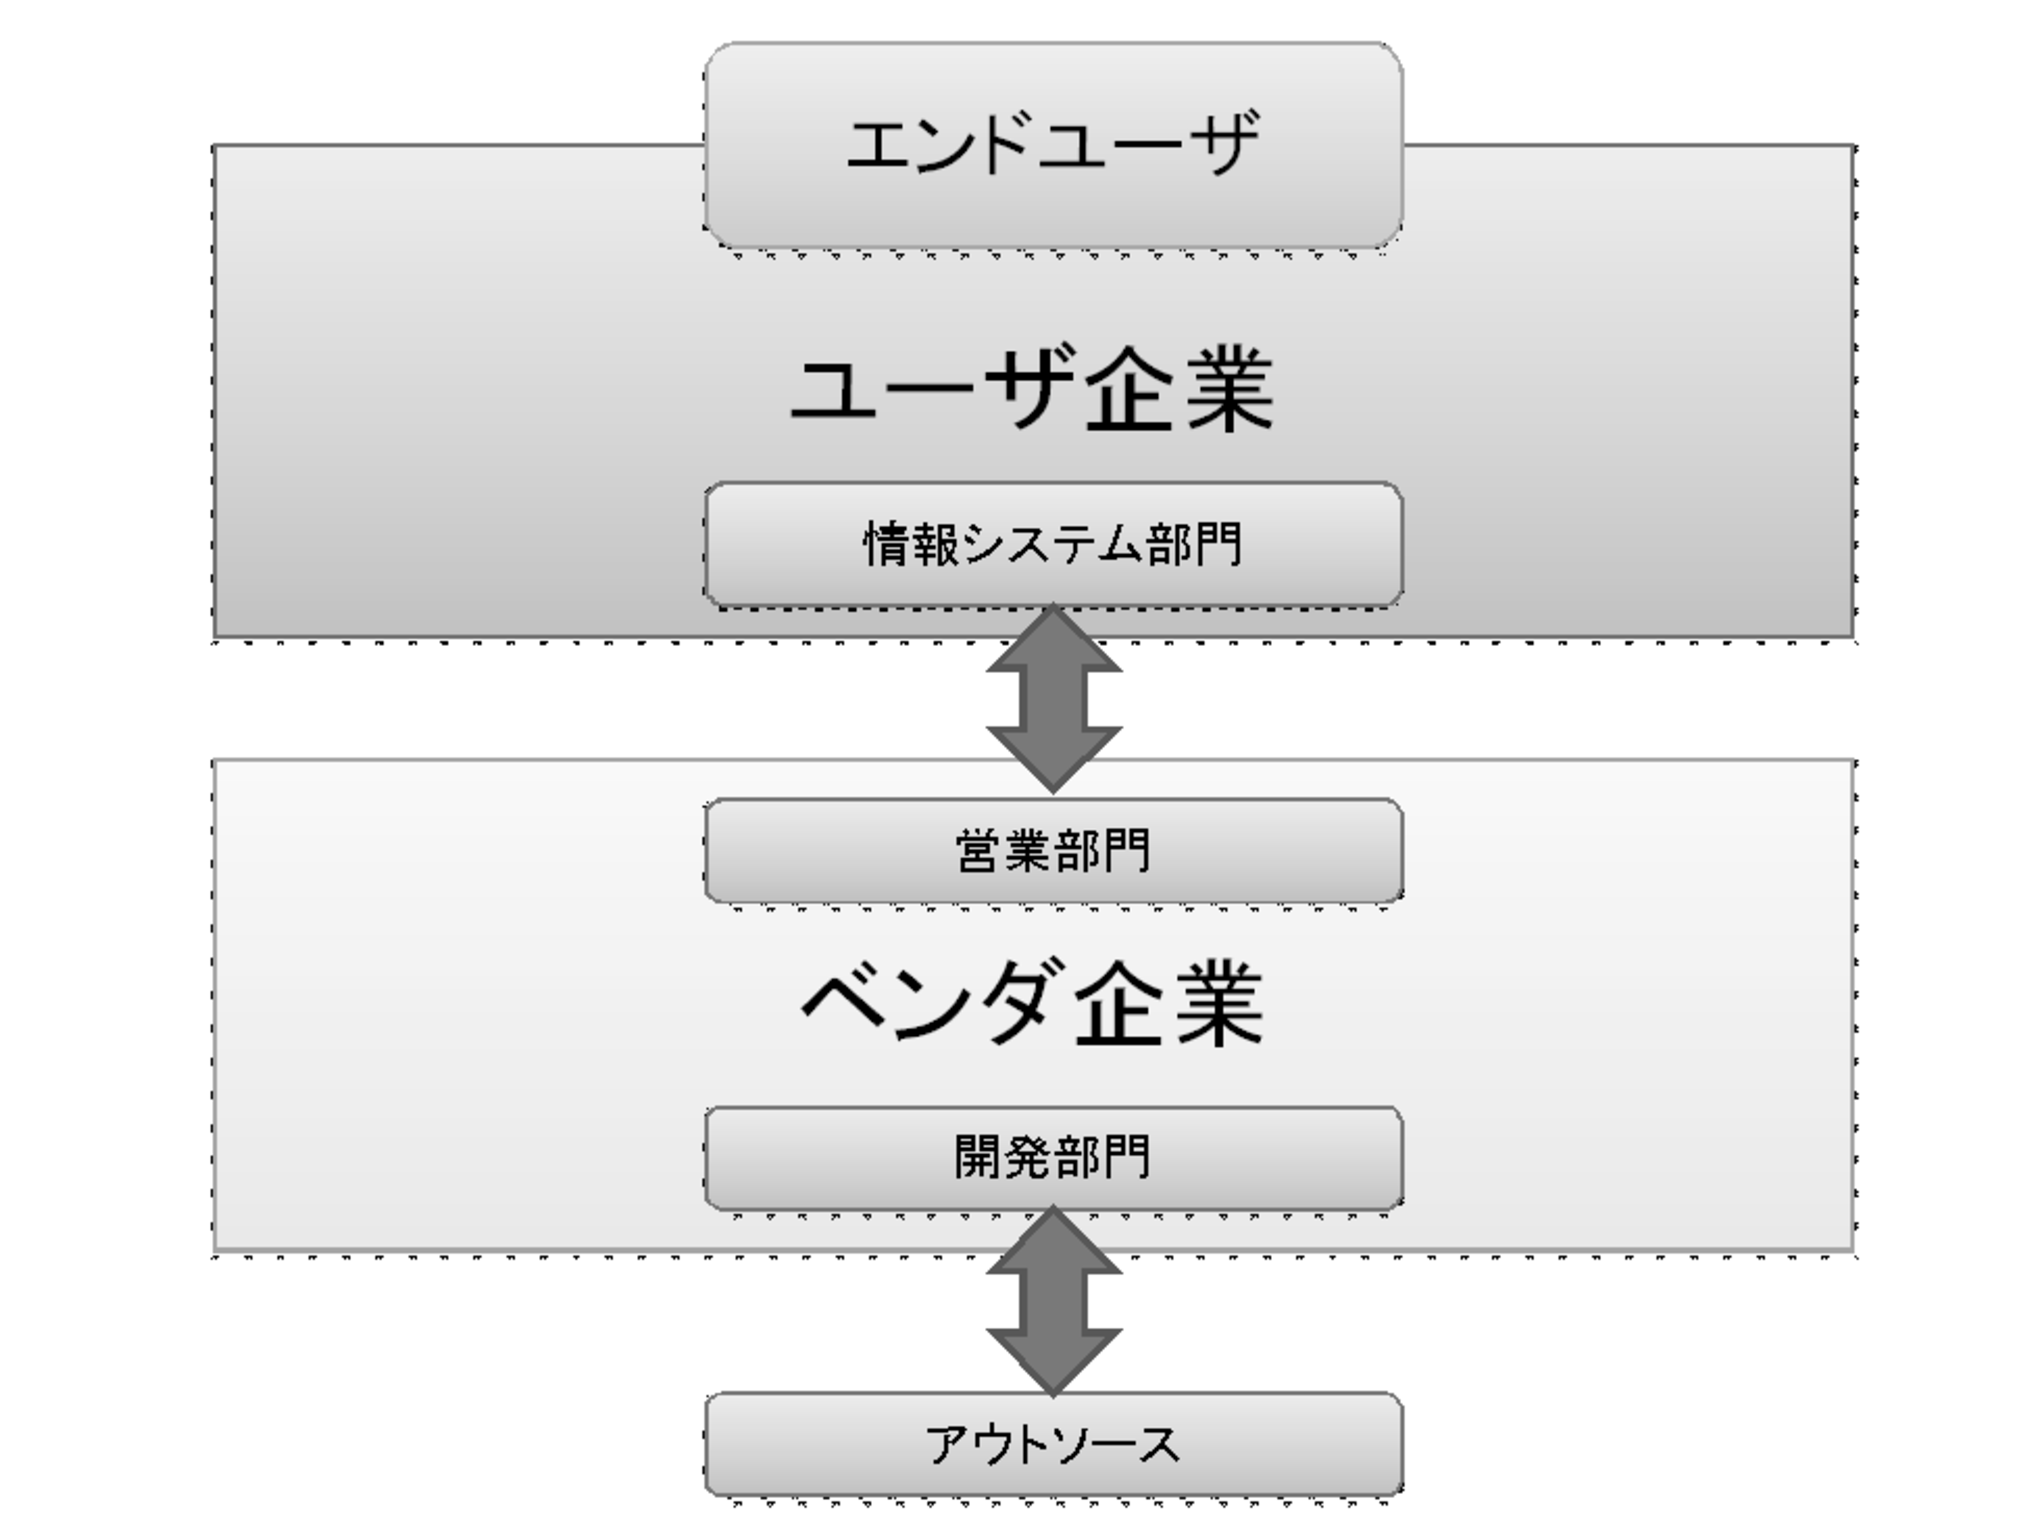
\includegraphics[width=7cm]{figs/user_vendor_model.eps}
		         \caption{ユーザ企業とベンダ企業の構造}
		         \label{fig:user_vendor_model}
	         \end{center}
         \end{wrapfigure}
    
    しかしながら,産業界に目を向けると,我が国においては,コ・クリエイティブにソフトウェアを開発することよりも,
    IT技術を提供するベンダ企業と,自社のサービスのためにIT技術を利用するユーザ企業との間には対立構造が明確に存在し,
    両者のコンフリクトをマネジメントすることがソフトウェア開発チームに求められてきた.
    
    図\ref{fig:user_vendor_model}は,従来のソフトウェア開発におけるユーザ企業とベンダ企業との関係構造を模式化したものである.
    一番上に示した「エンドユーザ」とは,実際にソフトウェアを利用するユーザ(個人)である.エンドユーザは「ユーザ企業」に所属し,
    企業が提供するサービスを実現するために情報システムを利用する.近年は,B2C型でサービスを提供する企業が増えたことから,
    エンドユーザはユーザ企業の外部に存在し,Web等でユーザ企業が提供するサービスを利用する場合も見られる.
    
    このようなソフトウェア開発を行う場合,一般的にユーザ企業にある「情報システム部門」がシステム開発を主導することになる.
    情報システム部門は複数の「ベンダ企業」に対してRFP(Request For Proposal)を提示し,これを受けてベンダが作成した
    提案を精査し,ソフトウェア開発を発注するベンダ企業を選定する.この一連のプロセスはベンダ企業の「営業部門」が担当する.
    
    営業部門が契約を取り付けた後,ベンダ企業の「開発部門」が実際のソフトウェア開発プロジェクトを開始することになる.
    このとき,ベンダ企業内で必要なリソースが調達できない場合,ベンダ企業は社外の企業等に対して「アウトソース」を行う.
    いわゆる下請けの関係であり,近年は人件費の安い海外にアウトソースすることも多い.
    
	\begin{flushleft}
		■IT産業の構造変化
	\end{flushleft}

    前項で述べたとおり,既存のソフトウェア開発の産業構造では,ソフトウェアを実際に開発しているチームと,
    ソフトウェアを利用するエンドユーザとの間に,幾つもの障壁があることがわかる.
    このような構造でソフトウェア開発を進めている限り,利用者が本当に望むソフトウェア製品が開発される可能性が
    低くなるのは自明のことである.
    ましてや,マーケットとの対話を通してコ・クリエイティブに製品開発を進めることなど,既存の構造では不可能である.
    
    翻って世界に目を向けると,以上述べてきたユーザとベンダ企業が対立する構造によらない,新しいインターネット企業が登場してきている.例えば,
    GoogleやFacebookなどの有力な企業は,自らの顧客であるユーザとインタネットを通じて直接的にコミュニケーションをしながら,
    自社のプロダクトとしての情報サービスを提供している.加えて,App StoreやGoogle Playといったスマートフォン向けアプリの
    マーケットが登場しており,個人であっても直接ソフトウェアプロダクトをマーケットに投入することさえ容易になってきた.
    よって,今後は,従来の情報産業の枠組みに当てはまらない新しいタイプの企業が成長してくるものと予測する.
    
	\begin{flushleft}
		■次世代のソフトウェア開発者育成手法としてのPBL
	\end{flushleft}

    このような状況を踏まえると,今後は従来型の「ユーザ・ベンダ型モデル」は急速に存在感を失い,代わりに,
    ソフトウェアを開発するチームが直接的にマーケットとの対話を行い,より良いサービスを開発し,市場でマネタイズするという,
    「コ・クリエイティブ型のソフトウェア開発モデル」がより一般的になるとの確信に至る.
    
    そこで,本研究ではこのような「コ・クリエイティブ型ソフトウェア開発」に対応できる知識や技術を持った人材を育成するための
    PBL型の教材と教授法について研究開発を行うことを目的とする.
    
    従来のPBLは
    図\ref{fig:user_vendor_model}におけるベンダー企業の技術者育成を主眼とするものがほとんどである.
    これでは,産業構造の変化を踏まえた次世代の開発者を育成する内容として不十分である.
    特に,マーケットとのコ・クリエイティブな対話のプロセス,及び,
    迅速にソフトウェアを開発するチームとしてのアジャイル性を獲得する方法などについて,深く学べる内容にする必要がある.
    
    以上の背景を踏まえ,次世代のソフトウェア開発者を育成するための
    「コ・クリエイティブなソフトウェア開発者を育成するPBL型教育」の手法を確立し,必要な教材やWebサービスとともにパッケージ化し,
    様々な教育機関における教育に提供できる成果を得ることを本研究の目的とする.
    
    
	\vspace{1cm}
	\begin{thebibliography}{99}
		\bibitem{wired} 顧客とのco-creationプラットフォーム-ベストプラクティ, 2012/10/24参照 \\
                        \tt{http://wired.jp/2011/09/29/}
	\end{thebibliography}
%end  研究目的 ====================
}

%====================================
%form: kiban_ab_form_03-05.tex ; user: kiban_ab_03-05_plan.tex
%========== S-1-7 基盤研究(A,B)(一般) =========
%===== p. 03-05 研究計画・方法 =============
\section{研究計画・方法}
%watermark: w08_plan_AB
\newcommand{\研究計画と方法概要}{%
%begin  研究計画と方法概要===================
	コ・クリエイティブなソフトウェア技術者を育成するために本研究で作成するPBL型の教材は,
	大きく,PBLの開始前に学生が前提知識を学習ための「事前学習教材」と,
	指導する教員向けの「指導手引書」からなる.これらは電子書籍として作成し,
	ビジュアルな表現により理解しやすいものとする.
	特に,ビデオ収録映像のクォリティを高めるために,教材製作のためのスタジオを用意し,
	業務用の機器を利用した収録環境を用意する.
	これとともに,学生のための「支援用情報システム」と教育効果の「測定用キット」も開発する.
	
	以上の研究は,本学や他大学でのPBL教育において随時利用することで改善し,完成度を高めるものとする.
	また,構築した情報システムはクラウド型のサービス上において運用し,広くこのPBL教育を実施したい利用者に
	提供するものとする.
    
%end  研究計画と方法概要 ====================
}

\newcommand{\研究計画}{%
%begin  研究計画===================
	
	\begin{flushleft}
		■研究全体の目標
	\end{flushleft}
	
	本研究は平成25年度から3カ年で実施し,全体を大きく次の目標に分割して取り組む.

	\begin{enumerate}
	    \item \label{enum:student} 学生用事前学習教材
		\item \label{enum:startup} PBL教材製作スタジオ
	    \item 教員向け指導手引書
	    \item 学習者支援用情報システム
	    \item 教育効果測定用キット
	    \item 成果発表
	\end{enumerate}
	
	このうち,\ref{enum:student}と\ref{enum:startup}を平成25年度に実施し,残りを平成26年度以降に実施する.
	
	% 半年ごとにサイクルを回す.リーンスタートアップを実施する.

	\begin{flushleft}
		■平成25年度の計画
	\end{flushleft}

	\underline{学生用事前学習教材}とは,PBLに入る前に事前に学習するための教材である.
	
	PBLでは,学生に事前の学習をするための教材が必要で,本研究者が実施した過去の例では
	いきなりソフトウェア開発プロジェクトを始めてもうまくいかない場合が多かった.
	そこで,本研究では学生に事前に準備のための学習をするための教材を	作成して提供する.
	
	コ・クリエイティブなソフトウェア開発者を育成するためのPBLの事前学習教材に含む内容は次のとおりとし,
	それぞれにInstructional Designを実施して学習者にとって理解しやすいように,ビジュアル面にも
	配慮したコンテンツとする.

	\begin{enumerate}
	  \item \label{enum:scrum} Agile型開発プロセス「Scrum」の方法論とツール
	  \item \label{enum:lean} リーン・スタートアップの概念と実施法
	\end{enumerate}
	

	\ref{enum:scrum}.のScrumとは,他のウォータフォールモデルや,
	RUP(Rational Unified Process)などの方式と比較して,軽量な
	ソフトウェア開発のための方法論であり,近年注目されている.
	

         \begin{wrapfigure}{r}{7cm}
     		% \vspace{-2.5cm}
         	\begin{center}
		         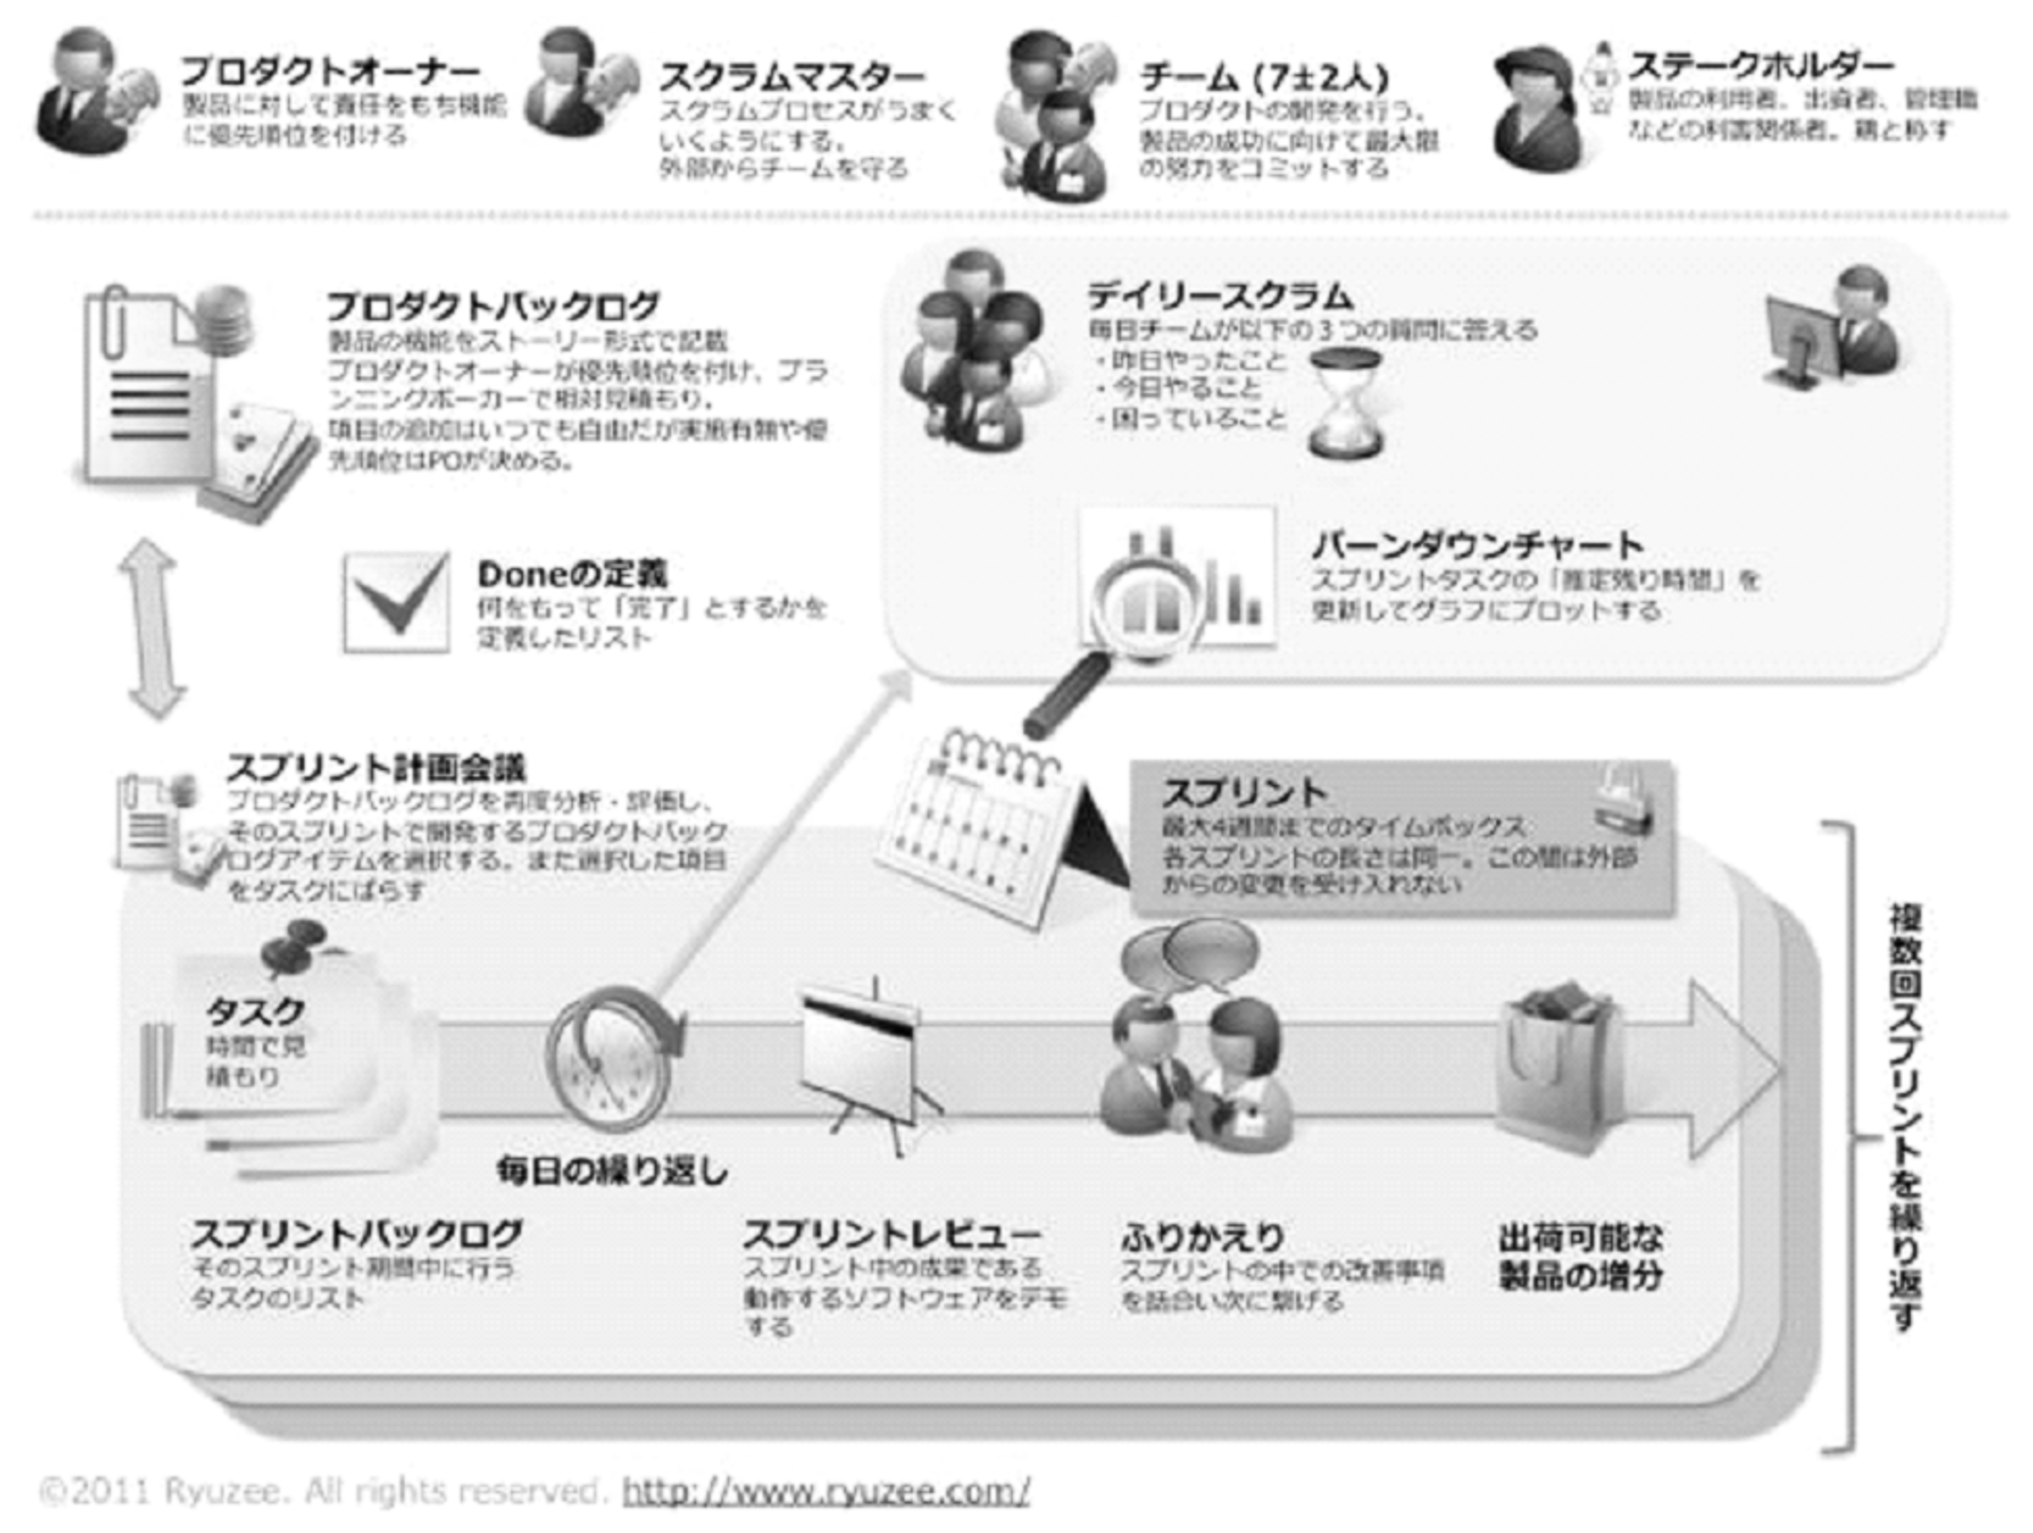
\includegraphics[width=7cm]{figs/scrum.eps}
		         \caption{Scrumの全体像(吉羽氏資料より)}
		         \label{fig:scrum}
	         \end{center}
         \end{wrapfigure}

	Scrumの全体像は図\ref{fig:scrum}でほぼ網羅されており,他の方式よりもシンプルであるため
	学習すべき知識の総量も少なくなる.しかしながら,実際には,単に知識として学ぶのではなく
	プロジェクトでScrumを実施できるようになるには相当の訓練が必要である.
	
	そこで,本研究で開発する教育法では
	知識項目を事前学習で学び,その後に続くPBLで実際にScrumをやってみることにより,Scrumで
	ソフトウェア開発を行うためのエッセンスを体得できるように工夫する.
	
	この教材に含む主要な内容は,Scrumの全体概要,
	役割分担(Scrum MasterやProduct Owner,Team Memberなど),
	成果物(プロダクトバックログ,スプリントバックログ,バーンダウンチャートなど),
	プロセス(スプリント計画会議,デイリースクラム,振り返りなど)についてである.
	加えて,Scrumで実際にソフトウェア開発を行うときに利用するクラウド型のツールについても解説する.
	また,本教材の内容についてはScrumコーチの認定資格を有する方にレビューして頂く.
	必要な学習時間は16~20時間を想定する.
	

	\ref{enum:lean}.のリーン・スタートアップとは,新しい製品・サービスを開発する際に
	利用できる方法論である.顧客にとって価値のないものを作ってしまうムダをなくし,
	時代が求める製品・サービスをより早く生み出すことができるのが特徴である\cite{lean-startup}.
	
	クラウド技術などの発展により,現在は作成したプロダクトをインターネット上のマーケットに投入することが
	従来と比べて容易になっている.よって,学生が実施するPBLの成果物を現実のマーケットで公開し,
	その評価を得ることも難しくなくなった.そこで,本研究で開発する教材では,リーン・スタートアップ型の
	開発方式に着目し,マーケットに受け入れられるソフトウェア・サービスを開発するために必要な知識を
	学べるようにする.これに要する学習時間は,8~10時間を想定する.

    
         \begin{wrapfigure}{r}{7cm}
         	\begin{center}
		         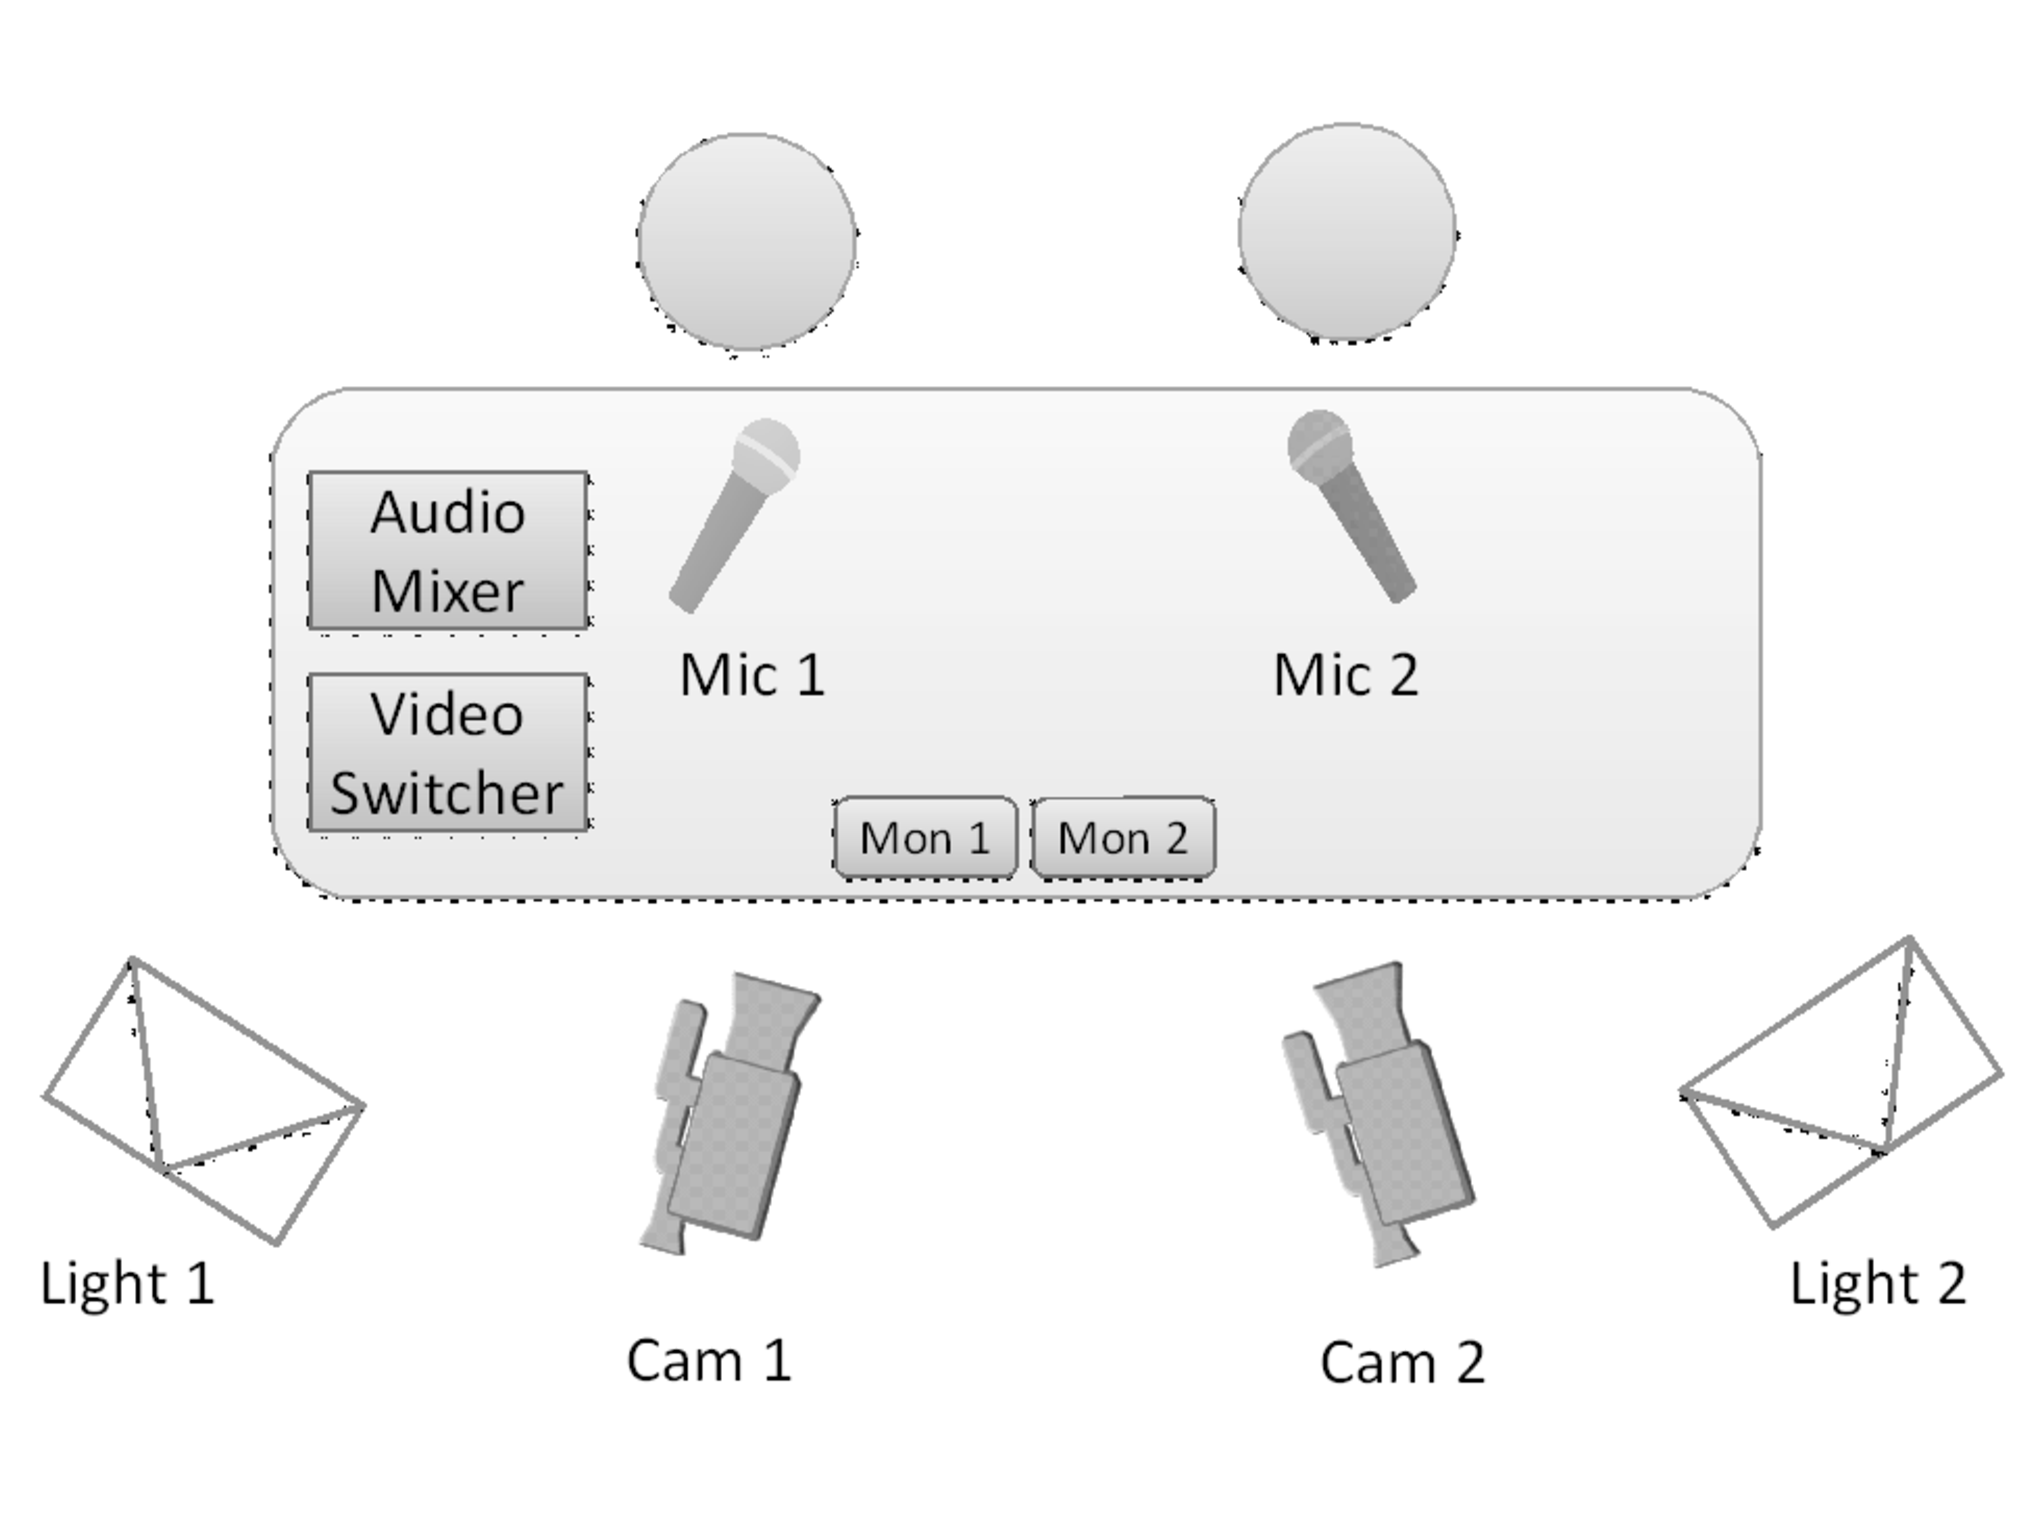
\includegraphics[width=7cm]{figs/studio.eps}
		         \caption{教材制作スタジオ}
		         \label{fig:studio}
	         \end{center}
         \end{wrapfigure}

	\vspace{0.5cm}
	\underline{PBL教材制作スタジオ}とは,本PBLで使用する教材製作のためのスタジオ環境である.
	本研究で作成する教材は,音声や動画を用いた電子書籍とする.
	そこで,電子書籍教材の製作に必要な映像・音響機器,及び,
	編集するためのコンピュータなどを購入して,本研究者の研究室に設置する.
	特に,作成する教材の映像・音響を収録のための機器は業務用クォリティ以上のものを選定する.
	図\ref{fig:studio}に示す通り、マイク、ビデオカメラ、ミキサ、スイッチャ、ライト等を配置し,
	教材製作のために使用する.
	
	\begin{flushleft}
		■平成26年度以降の計画
	\end{flushleft}
	
	\underline{教員用指導手引書}は,
	コ・クリエイティブなソフトウェア開発者育成を目的とするPBLを実施する教員などにむけたテキストである.
	
	このPBLの最大の特徴は,従来のウォータフォールモデルに即したPBLのように,
	情報システムの要求分析・設計・実装・テスト・運用という各工程を実施するためのスキルを学ぶのではなく,
	実際にプロダクトをマーケットに投入し,そのフィードバックを得て改善させ,
	よりユーザに受け入れられるソフトウェアとして高めていく作業を体験させることにある.
	
	そのため,教員はチームによる自己組織化の過程や,チームによる作業の改善プロセスの重要性を
	学生に指導しなくてはならない.これには,ゲーム感覚で取り組めるアンプラグドなワークショップを
	体験させるのが効果的である.そこで,この手引書には,各種のワークショップ(紙飛行機作成,ボール渡し,
	Manager-Workerゲームなど多数)を紹介し,実施するための方法について述べる.
	
	その他,チーム編成に再する注意点や,Scrum及びリーン・スタートアップの各プロセスについての指導法,
	成果発表会の運営や成績評価の方法,産学連携型で運営する場合の取り組み方などについてまとめる.
	
	\vspace{0.5cm}
	\underline{学習者支援用情報システム}は,PBL活動を行う学習者を支援するためのインフラストラクチャー
	であり,同時にScrum型の開発を行うための共同作業環境である.これには,ソースコードの構成管理,課題管理,
	Wikiやファイル共有といった基本機能に加え,これまでに作成した電子教材へもアクセスできるようにし,学生が
	演習時に必要に応じて参照できるようにする.
	このシステムは,オープンソースのプロダクトであるRedmineをベースに,本PBL教育向けに機能追加することで,
	クラウド型のLMSとして開発する予定である.

	\vspace{0.5cm}
	\underline{教育効果測定用キット}
	
	PBL学習の教育効果を定量的に測定することは一般的には非常に難しとされる.しかしながら,本研究で取り組むPBLを
	実施することにより,下記の項目を定量的に評価することができる.
	
	\begin{itemize}
	  \item マーケットからの反応(例:Facebookアプリの場合のいいねボタンを押された数,Google Playなどのアプリマーケットからのダウンロード数など)
	  \item 学生が取り組んだプロジェクトにおける詳細な課題とその完了数,及び作業時間(義捐用情報システムが記録する)
	  \item コラボレーションツールを用いたコミュニケーションの頻度
	\end{itemize}
	
	これらに加え,教員や外部の評価者からの意見などを加味し,学生のPBLでの教育効果を行うためのツールをまとめ,効果測定用キットとして
	パッケージにする.
	
	\vspace{0.5cm}
	\underline{成果発表}
	
	本研究で得た知見は,本学におけるPBL型授業や,他大学(慶應大学)の授業に随時導入し,その結果を積極的に発表する.
	発表する媒体としては,関連する学会等のほか,SNSやブログでも情報提供を行なっていく.
	これにより,本研究における成果を広く社会に還元するするものとする.
	
	また,作成した電子教材は各国語(英語,中国語・韓国語及びASEAN諸国の言語)に翻訳し,
	海外の技術者と日本の学生とが共同で取り組むことのできるグローバルなPBLへと展開していきたい.
	
	\vspace{1cm}
	\begin{thebibliography}{99}
		\bibitem{lean-startup} エリック・リース: リーン・スタートアップ ―ムダのない起業プロセスでイノベーションを生みだす, 日経BP社, 2012
	\end{thebibliography}

%end  研究計画 ====================
}

%form: kiban_ab_form_06.tex ; user: kiban_ab_06_preparation_final_year.tex
%========== S-1-7 基盤研究(A,B)(一般) =========
%===== p. 06 準備状況等、最終年度の応募 =============
\section{準備状況等、最終年度の応募}
\subsection{準備状況等}
\newcommand{\準備状況等}{%
%begin  準備状況等 ===================
	\underline{本研究を実施するための研究施設}としては,
	産業技術大学院大学(AIIT)では2006年度より情報システムのアーキテクトを育成するための
	PBLを実施しており(研究業績の\KLcite{pub:tozawa-pbl-2009}),本研究はこの一環として施設等を利用できる.
	また,このPBLにおいて,本研究者らはソフトウェア開発方法論を教育する目的で,
	反復型開発プロセスであるRUP(Rational Unified Process)や,XP(eXtreme Programming),チケット駆動開発などを
	指導した実績を有し,ここから得られた知見も活用する.
	特に,2009年度以降は,ベトナム国家大学の学生と共にグローバルPBLを展開し,
	海外の技術者との共同プロジェクトを実施し,その成果を発表している
	\KLcite{pub:kizaki-global-2011a}\KLcite{pub:kizaki-global-2011b}\KLcite{pub:kizaki-global-2011c}%
	\KLcite{pub:chubachi-global-2010}%
	\KLcite{pub:ohrui-global-2009}\KLcite{pub:tozawa-global-2009}.
	
	加えて,慶應義塾で開講している「協創型ソフトウェア開発」の授業を2011年度から担当し,今年度からは
	アジャイル型ソフトウェア開発手法であるScrumを全面的に導入し,コ・クリエイティブなソフトウェア開発者教育を始めたところである.

	\underline{本研究の研究成果を発信}するためには,AIITにおけるPBL全体を支援する情報インフラストラクチャに関する研究の成果
	\KLcite{pub:chubachi-ipbl-2012}\KLcite{pub:chubachi-ipbl-2011}%
	\KLcite{pub:chubachi-ipbl-2009a}\KLcite{pub:chubachi-ipbl-2009b}
	を活用する.
%end  準備状況等 ====================
}

\subsection{研究計画最終年度の応募}
\newcommand{\研究計画最終年度の応募の研究種目名}{%
%begin  研究種目名 ===================
         % 基盤研究A
%end  研究種目名 ====================
}

\newcommand{\研究計画最終年度の応募の審査区分}{%
%begin  審査区分 ===================
	%123
%end  審査区分 ====================
}

\newcommand{\研究計画最終年度の応募の課題番号}{%
%begin  課題番号 ===================
    %12345678	%半角(英数字)
%end  課題番号 ====================
}

\newcommand{\研究計画最終年度の応募の研究課題名}{%
%begin  研究課題名 ===================
	%シロナガスクジラの卵の殻はなぜ見つからないのか
%end  研究課題名 ====================
}

\newcommand{\研究計画最終年度の応募の研究期間初年度}{%
%begin  研究期間初年度 ===================
	%15
%end  研究期間初年度 ====================
}

\newcommand{\研究計画最終年度の応募の計画と成果}{%
%begin  特別推進研究又は基盤研究による研究計画及び研究成果 ===================
	%研究課題の通り、シロナガスクジラの卵は見つけられなかった。
%end  特別推進研究又は基盤研究による研究計画及び研究成果 ====================
}

\newcommand{\研究計画最終年度の応募の理由}{%
%begin  研究計画最終年度前年度の応募をする理由 ===================
	%さっさと次の研究に移りたいので。
%end  研究計画最終年度前年度の応募をする理由 ====================
}

%====== end of page =====================================
%form: kiban_ab_form_07-09.tex ; user: kiban_ab_07-09_publications.tex
%========== S-1-7 基盤研究(A,B)(一般) =========
%===== p. 07-09 研究業績 =============
\section{研究業績}
%watermark: w14_pub_AB
% 2012-09-01 Taku
\newcommand{\年と名前と研究業績}{%
%begin  研究業績 ===================
		% 2013年度から始まった2カラムのtabularです。
%ーーーーーーーーーーーーーーーーーーーーーーーーーーーーーーーーーーーーーーーーーーーー
%		\KLcite{pub:theoegg} のようにして業績番号を文中に入れられます。
%ーーーーーーーーーーーーーーーーーーーーーーーーーーーーーーーーーーーーーーーーーーーー
	2012 {\small 以降} \\
		中鉢欣秀
		& \KLbibitem \label{pub:chubachi-ipbl-2012} \me, 小山裕司: AIITにおけるプロジェクト型学修(PBL)のためのBacklogシステムの導入, 情報処理学会 第19回IOT・第39回EVA合同研究発表会, 島根県松江市, 2012-09-27\\ 
	\hline%----------------------------------------------
	
	2011 \\
		中鉢欣秀
		& \KLbibitem \label{pub:chubachi-ipbl-2011}\me, 小山 裕司: PBLを支援するコラボレーティブツールに関する考察, 産業技術大学院大学紀要, No.5,pp.100-108, 2011 (査読有)\\
		% & \KLbibitem 小山 裕司, \me: 外部アカウント認証を使った本人確認付き利用者認証の仕組み, 産業技術大学院大学紀要, No.5,pp.75-80, 2011(査読有) \\
		& \KLbibitem \me: 目的/手段展開に基づくソフトウェアアーキテクチャの仕様化, 要求工学WGワークショップ, 情報処理学会, 礼文島, 2011-06-24 \\
		& \KLbibitem \label{pub:kizaki-global-2011a} 木崎 悟, 成田 亮, 丸山 英通, \me: グローバルなソフトウェア開発におけるマネジメント手法, 情報処理学会 第172回ソフトウェア工学研究会, 早稲田大学, 2011-05-17 \\
		& \KLbibitem \label{pub:kizaki-global-2011b} 木崎 悟, 成田 亮, 丸山 英通, 土屋 陽介, 成田 雅彦, \me: 国際PBLにおける的確な仕様の伝達とチケット駆動による開発作業の効率化, ソフトウェアエンジニアリングシンポジウム2011, 東京女子大学, 2011-09. \\
		& \KLbibitem \label{pub:kizaki-global-2011c} 木崎 悟, 丸山 英通, 土屋 陽介, \me: ソフトウェア開発PBLへのチケット駆動開発の適用による共同作業の改善, プロジェクトマネジメント学会 2011年度秋季研究発表大会, 産業技術大学院大学, 2011-09. \\
		& \KLbibitem 小山 裕司, \me, 土屋 陽介: ソーシャルメディアを活用したコネクション構築支援, 情報処理学会研究報告. コンピュータと教育研究会報告, 一般社団法人情報処理学会, Vol.2011, No.3, pp.1-6, 2011-12-10. \\
		& \KLbibitem 土屋 陽介, 小山 裕司, \me: 授業配信システムの設計と開発, 情報処理学会研究報告. コンピュータと教育研究会報告, 一般社団法人情報処理学会, Vol.2011, No.2, pp. 1-7, 2011-12-10. \\
		& \KLbibitem \me, 小山 裕司, 石島 辰太郎: 産業技術大学院大学のICT環境の運用と課題, 研究報告インターネットと運用技術(IOT), 一般社団法人情報処理学会, Vol.2012-IOT-16, No.11, pp.1-4, 2012-03-08 \\

	\hline%----------------------------------------------
	2010 \\
		中鉢欣秀
		&  \KLbibitem \label{pub:chubachi-global-2010} \me, 成田 雅彦, 戸沢 義夫: 加藤由花, 戸沢義夫: ベトナム国家大学とのグローバル PBL から得た知見, 産業技術大学院大学紀要, pp.1-4, 2010 (査読有) \\
		&  \KLbibitem S.~Ishijima, H.~Koyama, \meen, F.~Harashima: ICT-based Learning System of AIIT for the professional education in Japan, 9th International Conference on Information Technology Based Higher Education and Training (ITHET 2010), 2010-04-29 \\
		&  \KLbibitem R.~Nishino, M.~Kojima, O.~Oka, T.~Okino, T.~Sugita, Y.~Tsuchiya, H.~Koyama, Y.~Tozawa, \meen: Experience Gained through International PBL in Software Development, 1st Asia-Pacific Joint PBL Conference 2010, 2010-10-23 \\
		&  \KLbibitem \meen, Y.~Kato, Y.~Tozawa: Web-based groupware supporting PBL effectively, 1st Asia-Pacific Joint PBL Conference 2010, 2010-10-24 \\
		&  \KLbibitem \me: ワークショップ実行委員長業務のSBVA法による要求分析, 要求工学ワーキンググループ ワークショップ, 情報処理学会, 礼文島, 2010-06-17 \\
		&  \KLbibitem 木崎 悟, 成田 亮, 丸山 英通, \me, 長尾 雄行: GTD初心者のタスク管理を支援するタスクコンシェルジュの開発, 第9回情報科学技術フォーラム, 福岡県福岡市, 2010-08-20 \\
		&  \KLbibitem \me, 小山 裕司, 石島 辰太郎: ICTを基盤とした高度専門職教育, 情報教育シンポジウム論文集, 情報処理学会, 情報処理学会シンポジウムシリーズ IPSJ Symposium Series Vol.2010, No.6, pp.133-138, 群馬県渋川市, 2010-08-19 \\
		&  \KLbibitem \me: 遠隔会議システムを用いた国際PBLから得た知見, 日本e-Learning学会 2010年度学術講演会論文誌, 東京都千代田区, 2010-11-14 \\
		&  \KLbibitem 木崎 悟, 成田 亮, 丸山 英通, 土屋陽介, \me: タスク管理を支援するタスクコンシェルジュの開発, 電子情報通信学会総合大会ポスターセッション, 東京都市大学, 2011-03-16. \\

	\hline%----------------------------------------------

	2009 \\
		中鉢欣秀
		 &  \KLbibitem \label{pub:chubachi-ipbl-2009a} \me, 土屋 陽介, 長尾 雄行, 加藤 由花, 酒森 潔, 戸沢 義夫: グループウェア導入によるPBLの見える化, 日本e-Learning学会論文誌, Vol.9, pp.129-135, 2009-05(査読有) \\
		 &  \KLbibitem \label{pub:chubachi-ipbl-2009b} \me, 加藤由花, 戸沢義夫: PBL用情報インフラストラクチャの構築と運用, 産業技術大学院大学紀要, pp.109-116, 2009 (査読有) \\
		 &  \KLbibitem \label{pub:tozawa-pbl-2009} Y.~Tozawa, Y.~Kato, \meen: Efforts to ensure the quality of PBL education in the graduate school of Information Technology, Proceedings of the 2nd International Research Symposium on PBL, 3-4 December 2009, Melbourne, Australia, pp.1-9 \\
		 &  \KLbibitem \label{pub:ohrui-global-2009} 大類 優子,成田 雅彦,\me,土屋 陽介,戸沢 義夫: Global PBL Feasibility Studyの実践検証, 情報科学技術フォーラム講演論文集, FIT(電子情報通信学会・情報処理学会)推進委員会, 2009-08-20, Vol.8, No.4, pp. 515-516 \\
		 &  \KLbibitem \me: 要求記述演習によるロジカルシンキング教育の評価, 要求工学ワーキンググループ ワークショップ, 情報処理学会, 銚子, 2009-05-29 \\
		 &  \KLbibitem \label{pub:tozawa-global-2009} 戸沢 義夫, 成田 雅彦, \me, 土屋 陽介: Global PBL Feasibility Studyの実践と得られた知見, 情報処理学会 情報教育シンポジウム論文集, pp.167-174,2009-08-20 \\
		 &  \KLbibitem \me: 要求分析モデリング支援システムの開発~SBVAエディタ~, 要求工学ワーキンググループ ワークショップ, 情報処理学会, 天橋立, 2009-10-22 \\
		 % &  \KLbibitem \me: 要求工学セッションの紹介~WW2010~, ウィンターワークショップ2010イン・倉敷論文集,情報処理学会,情報処理学会シンポジウムシリーズ IPSJ Symposium Series Vol.2010,No.3, pp.31-32, 2010-01-21 \\

	\hline%----------------------------------------------

	2008 \\
		中鉢欣秀
		&  \KLbibitem 長尾 雄行, 土屋 陽介, 森本 祥一, \me: JavaScriptと非同期HTTPリクエストによる共同作業支援ミドルウェアの構築, 産業技術大学院大学紀要, Vol.2, pp.165-174, 2008 \\
		&  \KLbibitem 森本 祥一, \me: シナリオの図解化による業務フロー分析, 産業技術大学院大学紀要, Vol.2, pp.193-208, 2008 \\
		&  \KLbibitem \me, 専門職大学院におけるモデリング教育とSBVA法, 要求工学ワーキンググループ ワークショップ, 情報処理学会, 奄美大島, 2008-05-15 \\
		&  \KLbibitem 長尾 雄行, 土屋 陽介, 森本 祥一, \me: JavaScriptと非同期HTTPリクエストによる共同作業支援ミドウェアの構築, 情報処理学会論文誌:プログラミング, Vol.1, No. 1, pp.63-64, 2008-06 \\
		&  \KLbibitem \me, システム開発における仮説検証型の要求分析プロセス, 要求工学ワーキンググループ ワークショップ, 情報処理学会, 雲仙, 2008-10-23 \\
		&  \KLbibitem \me, 土屋 陽介, 長尾 雄行, 加藤 由花, 酒森 潔, 戸沢 義夫, PBLを見える化する協調作業支援環境の構築, 日本e-Learning学会2008年秋季学術講演会論文集, pp.72-79, 京都, 2008-11 ※優秀賞受賞 \\
		&  \KLbibitem \me: 要求分析者育成のためのコミュニケーション能力教育, ウィンターワークショップ2009・イン・宮崎論文集, 情報処理学会, Vol.2009, No.3, pp.45-46, 宮崎, 2009-01-23 \\
		% &  \KLbibitem 橋山 牧人,中鉢 欣秀, 大岩 元: 携帯ゲームアプリケーション開発を支援するオブジェクト指向を用いたフレームワークの開発, 情報処理学会第71会全国大会, pp.4-733-734,草津(滋賀), 2009年3月 (NII)
%end  研究業績  ====================
}

\newcommand{\連携研究者の研究業績}{%
%begin  連携研究者の研究業績 ===================
		% 2カラムのtabularです。
%ーーーーーーーーーーーーーーーーーーーーーーーーーーーーーーーーーーーーーーーーーーーー
%		\KLciteB{pub:theoegg} のようにして業績番号を文中に入れられます。
%ーーーーーーーーーーーーーーーーーーーーーーーーーーーーーーーーーーーーーーーーーーーー
%end  連携研究者の研究業績  ====================
}

%===========================================================
 %=======================================================
%form: kiban_ab_form_10.tex ; user: kiban_ab_10_past_funds.tex
%========== S-1-7 基盤研究(A,B)(一般) =========
%===== p. 10 これまでに受けた研究費とその成果等 =============
\section{これまでに受けた研究費とその成果等}
\newcommand{\これまでに受けた研究費とその成果等}{%
%begin  これまでに受けた研究費とその成果等 ===================
	\begin{itemize}
		\item 若手研究(B) ,2008~2009年度,
		    「情報システムアーキテクト育成のための遠隔教育システム」,研究代表者,3,900千円\\
		    本研究では社会人教育における利用を想定したモデリング遠隔教育支援シス
            テムを研究開発した.これを用いて,特にユーザ企業の社会人を対象としたモデリング
            教育支援環境を構築し,その有用性を確かめることができた.
    \end{itemize}
%end  これまでに受けた研究費とその成果等 ====================
}

%====== end of page =====================================
%form: kiban_ab_form_11.tex ; user: kiban_ab_11_relation.tex
%========== S-1-7 基盤研究(A,B)(一般) =========
%===== p. 11 研究計画と研究進捗評価を受けた研究課題の関連性 =============
\section{研究計画と研究進捗評価を受けた研究課題の関連性}
\newcommand{\研究計画と研究進捗評価を受けた研究課題の関連性}{%
%begin  研究計画と研究進捗評価を受けた研究課題の関連性 ===================
	特になし.
%end  研究計画と研究進捗評価を受けた研究課題の関連性 ====================
}

%====== end of page =====================================
%form: kiban_ab_form_12.tex ; user: kiban_ab_12_human_rights_etc.tex
%========== S-1-7 基盤研究(A,B)(一般) =========
%===== p. 12 人権、法令、研究経費の妥当性など =============
\section{人権、法令、研究経費の妥当性など}
\newcommand{\人権の保護及び法令等の遵守への対応}{%
%begin  人権の保護及び法令等の遵守への対応 ===================
	特になし.
%end  人権の保護及び法令等の遵守への対応 ====================
}

\subsection{研究経費の妥当性・必要性}
\newcommand{\研究経費の妥当性と必要性}{%
%begin  研究経費の妥当性・必要性 ===================
	「研究計画・方法」欄で述べた研究内容を踏まえ,
	設備備品費は,初年度に教材製作スタジオを構築するための費用を支出し,	以降,
	動画編集用PCと動画配信用PCを各年度に購入する.

	消耗品費は,本研究に関連する書籍代・文具代などにあてる.

	国内旅費については,国内の他の教育機関で実施しているソフトウェア開発系PBLの調査と学会発表の旅費として用いる.
	外国旅費についても海外のPBL動向調査及び国際学会への旅費・参加費とする.
	
	本研究で製作をする教材の作成作業を補助するためのアルバイトを1名雇用する(月額80,000円程度).
	また,本研究の内容についてScrumの専門家(コーチ)への協力を依頼し,レビュー等をしていただくための
	謝金を用意する.
	
	また,教材へのナレーションを吹き込む専門のナレータへの謝金の支出を予定する.
	研究の2年目から,システム開発をするためのエンジニアを雇用するための謝金が必要になる(月額100,000円程度).
	研究の最終年度には,教材の評価への協力や,教材翻訳のための謝金を用意する.
	
	その他として,通信費を計上する.
%end  研究経費の妥当性・必要性 ====================
}

%====== end of page =====================================
%form: kiban_ab_form_13.tex ; user: kiban_ab_13_materials.tex
%========== S-1-7 基盤研究(A,B)(一般) =========
%===== p. 13 設備備品費、消耗品費の明細 =============
\section{設備備品費、消耗品費の明細}
%				\KLJFY{\1年目J}
\newcommand{\設備備品費1年目}{%
%begin  設備備品費1年目 ===================
	\KLItemNumUnitCostLocation{卓上マイク}{2}{35}{産技大}
	\KLItemNumUnitCostLocation{音響ミキサー}{1}{60}{産技大}
	\KLItemNumUnitCostLocation{音響用ケーブル一式}{1}{100}{産技大}
	\KLItemNumUnitCostLocation{ビデオカメラ}{2}{115}{産技大}
	\KLItemNumUnitCostLocation{ビデオカメラスタンド}{2}{40}{産技大}
	\KLItemNumUnitCostLocation{映像用スイッチャ}{1}{120}{産技大}
	\KLItemNumUnitCostLocation{映像用モニタ}{2}{45}{産技大}
	\KLItemNumUnitCostLocation{スタンド式ライト}{2}{60}{産技大}
	\KLItemNumUnitCostLocation{動画記録用PC}{2}{150}{産技大}
%end  設備備品費1年目 ====================
}

\newcommand{\消耗品費1年目}{%
%begin  消耗品費1年目 ===================
	% 2カラムのtabularです。
	\KLItemCost{書籍代}{100}
	\KLItemCost{文具代}{100}
	\KLItemCost{OA用品代}{100}
	\KLItemCost{記録用媒体}{100}
%end  消耗品費1年目 ====================
}

\newcommand{\設備備品費2年目}{%
%begin  設備備品費2年目 ===================
	\KLItemNumUnitCostLocation{動画編集用PC}{1}{150}{産技大}
%end  設備備品費2年目 ====================
}

\newcommand{\消耗品費2年目}{%
%begin  消耗品費2年目 ===================
	\KLItemCost{書籍代}{100}
	\KLItemCost{文具代}{100}
	\KLItemCost{OA用品代}{100}
	\KLItemCost{記録用媒体}{100}
%end  消耗品費2年目 ====================
}

\newcommand{\設備備品費3年目}{%
%begin  設備備品費3年目 ===================
	\KLItemNumUnitCostLocation{動画配信用PC}{1}{150}{産技大}
%end  設備備品費3年目 ====================
}

\newcommand{\消耗品費3年目}{%
%begin  消耗品費3年目 ===================
	\KLItemCost{書籍代}{100}
	\KLItemCost{文具代}{100}
	\KLItemCost{OA用品代}{100}
	\KLItemCost{記録用媒体}{100}
%end  消耗品費3年目 ====================
}

%====== end of page =====================================
%form: kiban_ab_form_14.tex ; user: kiban_ab_14_travels.tex
%========== S-1-7 基盤研究(A,B)(一般) =========
%===== p. 14 旅費等の明細 =============
\section{旅費等の明細}
%	\KLNoMarginMinipage{66}{706}{566}{
%				\KLJFY{\1年目J}
\newcommand{\国内旅費1年目}{%
%begin  国内旅費1年目 ===================
		% 2カラムのtabularです。
		\KLItemCost{PBL動向調査}{100}
		\KLItemCost{学会発表}{100}
%end  国内旅費1年目 ====================
}

\newcommand{\外国旅費1年目}{%
%begin  外国旅費1年目 ===================
		% 2カラムのtabularです。
		\KLItemCost{PBL動向調査}{350}
		\KLItemCost{国際会議発表}{400}
%end  外国旅費1年目 ====================
}

\newcommand{\謝金等1年目}{%
%begin  謝金等1年目 ===================
		% 2カラムのtabularです。
	 	\KLItemCost{アルバイト報酬(教材製作補助等)}{960}
		\KLItemCost{謝金(Scrumコーチ等)}{800}
%end  謝金等1年目 ====================
}

\newcommand{\その他1年目}{%
%begin  その他1年目 ===================
		% 2カラムのtabularです。
	 	\KLItemCost{通信費}{120}
%end  その他1年目 ====================
}

\newcommand{\国内旅費2年目}{%
%begin  国内旅費2年目 ===================
		% 2カラムのtabularです。
		\KLItemCost{PBL動向調査}{100}
		\KLItemCost{学会発表}{200}
%end  国内旅費2年目 ====================
}

\newcommand{\外国旅費2年目}{%
%begin  外国旅費2年目 ===================
		% 2カラムのtabularです。
		\KLItemCost{PBL動向調査}{300}
		\KLItemCost{国際会議発表}{400}
%end  外国旅費2年目 ====================
}

\newcommand{\謝金等2年目}{%
%begin  謝金等2年目 ===================
	 	\KLItemCost{アルバイト報酬(教材製作補助等)}{960}
		\KLItemCost{謝金(Scrumコーチ等)}{800}
		\KLItemCost{謝金(システム開発)}{1200}
%end  謝金等2年目 ====================
}

\newcommand{\その他2年目}{%
%begin  その他2年目 ===================
	 	\KLItemCost{通信費}{120}
%end  その他2年目 ====================
}

\newcommand{\国内旅費3年目}{%
%begin  国内旅費3年目 ===================
		% 2カラムのtabularです。
		\KLItemCost{PBL動向調査}{100}
		\KLItemCost{学会発表}{300}
%end  国内旅費3年目 ====================
}

\newcommand{\外国旅費3年目}{%
%begin  外国旅費3年目 ===================
		% 2カラムのtabularです。
		\KLItemCost{PBL動向調査}{200}
		\KLItemCost{国際会議発表}{400}
%end  外国旅費3年目 ====================
}

\newcommand{\謝金等3年目}{%
%begin  謝金等3年目 ===================
	 	\KLItemCost{アルバイト報酬(教材製作補助等)}{960}
		\KLItemCost{謝金(Scrumコーチ等)}{800}
		\KLItemCost{謝金(教材評価)}{200}
		\KLItemCost{謝金(教材翻訳)}{200}
		\KLItemCost{謝金(システム開発)}{800}
%end  謝金等3年目 ====================
}

\newcommand{\その他3年目}{%
%begin  その他3年目 ===================
	 	\KLItemCost{通信費}{120}
%end  その他3年目 ====================
}

%====== end of page =====================================
%form: kiban_ab_form_15.tex ; user: kiban_ab_15_other_applications.tex
%========== S-1-7 基盤研究(A,B)(一般) =========
%===== p. 15 研究費の応募・受入等の状況・エフォート =============
\section{研究費の応募・受入等の状況・エフォート}
\subsection{応募中の研究費}
\newcommand{\本人の研究経費}{%
%begin  本人の研究経費 ===================
	\KLMyBudget{}{}% 初年度と、期間全体で「本人が」使う額
%	分担者がいない場合は、\KLMyBudget{}{} のように{}の中を空にしてください。金額が自動的に入ります。
%end  本人の研究経費  ====================
}

\newcommand{\応募中の研究費}{%
%begin  応募中の研究費 ===================
		%6カラムのtabular
		% 1:資金制度・研究費名(研究期間・配分機関名)
		% 2:研究課題名(研究代表者氏名)
		% 3:代表/分担
		% 4:初年度の研究経費(期間全体の額)
		% 5:エフォート
		% 6:研究内容の相違点及び他の研究費に加えて本応募研究課題に応募する理由
%		\multicolumn{6}{c}{\dotfill} \\
		
		
%end  応募中の研究費 ====================
}

%====== end of page =====================================
%form: kiban_ab_form_16.tex ; user: kiban_ab_16_other_funds.tex
%========== S-1-7 基盤研究(A,B)(一般) =========
%===== p. 16 受け入れ予定の研究費 =============
\subsection{受け入れ予定の研究費}
%    \KLNoMarginMinipage{\KLLeftEdge}{694}{568}{
\newcommand{\受け入れ予定の研究費}{%
%begin  受け入れ予定の研究費 ===================
%		\multicolumn{6}{c}{\dotfill} \\
%end  受け入れ予定の研究費 ====================
}

%====== end of page =====================================
%\KLCheckPageLimit
%\KLAdvancePages
% hook9 : right before \end{document} ============

%endUserFiles
% hook7 : right before including forms ============
 % for future maintenance

% kiban_ab_forms
%=======================================
\ifthenelse{\boolean{BudgetSummary}}{
	\KLTypesetPage{13}
	\KLTypesetPage{14}
}{}
	
\ifthenelse{\boolean{BudgetSummary}\OR \boolean{klTypesetPage0}}{
	%============================================================
%  Warning cover page
%============================================================

\begin{picture}(0,0)(\KLOddPictureX,\KLPictureY)
	\KLParbox{100}{700}{550}{600}{t}{
		\LARGE
		提出前に次の行を以下のようにコメントアウトし、\\
		コンパイルし直してください。\\
		\hspace{2cm}\%\textbackslash setboolean\{BudgetSummary\}\{true\}\\
		\hspace{2cm}\%\textbackslash KLTypesetPage\{..\}\\
		\hspace{2cm}\%\textbackslash KLTypesetPagesInRange\{..\}\{..\}\\
	}
	\西暦
	\KLParbox{100}{550}{500}{500}{t}{
		\begin{center}
			\LARGE 予算と研究組織のまとめ \\
			\Large \today
		\end{center}
	}

	\KLTextBox{100}{500}{550}{300}{}{
		\Large
		研究種目: \研究種目\研究種別\研究種目後半\\
		研究期間: \研究開始年度(H\研究開始元号年度) 〜 H\研究期間の最終元号年度\\
		研究課題名:「\研究課題名」\\
		研究代表者:\研究代表者氏名\\
		研究機関名:\研究機関名\\
	}
\end{picture}
\clearpage


}{}

\KLInputIfPageInRangeIsSelected{1}{2}{forms/kiban_ab_form_01-02}
\KLInputIfPageInRangeIsSelected{3}{5}{forms/kiban_ab_form_03-05}
\KLInputIfSelected{6}{forms/kiban_ab_form_06}
\KLInputIfPageInRangeIsSelected{7}{9}{forms/kiban_ab_form_07-09}
\KLInputIfSelected{10}{forms/kiban_ab_form_10}
\KLInputIfSelected{11}{forms/kiban_ab_form_11}
\KLInputIfSelected{12}{forms/kiban_ab_form_12}
\KLInputIfSelected{13}{forms/kiban_ab_form_13}
\KLInputIfSelected{14}{forms/kiban_ab_form_14}

\ifthenelse{\boolean{BudgetSummary}}{
	% Print the Grand Total of the budget to the console. (as requested by the Kakenhi-Macro group).
\KLPrintGrandTotal

%==== Summary Table in DRAFT mode =====
\ifthenelse{\boolean{BudgetSummary}}{
	\newpage
	
	% restore parameters
	\setlength{\topmargin}{-2cm}
	\setlength{\oddsidemargin}{-0.5cm}
	\setlength{\evensidemargin}{-0.5cm}
	\setlength{\textwidth}{16cm}
	\setlength{\linewidth}{16cm}
	\setlength{\textheight}{25cm}

	\newpage	
	%==================================================
\phantom{x}	\vspace{1cm}
\begin{tabular}{r|r|rrrrr}
	\multicolumn{7}{r}{(金額単位:千円)}\\
	\hline
	年度 & 年度合計 & 設備備品 & 消耗品 &旅費 & 謝金等 & その他\\
	\hline
	\1年目西暦(H\1年目) & 
		\NumC{KLAnnualSum1} &
		\NumC{KLequipments1} & \NumC{KLexpendables1} & 
		\NumC{KLtravel1} & \NumC{KLgratitude1} & \NumC{KLmisc1}\\
	\hline
	\2年目西暦(H\2年目) & 
		\NumC{KLAnnualSum2} &
		\NumC{KLequipments2} & \NumC{KLexpendables2} & 
		\NumC{KLtravel2} & \NumC{KLgratitude2} & \NumC{KLmisc2}\\
	\hline
	\3年目西暦(H\3年目) & 
		\NumC{KLAnnualSum3} &
		\NumC{KLequipments3} & \NumC{KLexpendables3} & 
		\NumC{KLtravel3} & \NumC{KLgratitude3} & \NumC{KLmisc3}\\
	\hline
	\4年目西暦(H\4年目) & 
		\NumC{KLAnnualSum4} &
		\NumC{KLequipments4} & \NumC{KLexpendables4} & 
		\NumC{KLtravel4} & \NumC{KLgratitude4} & \NumC{KLmisc4}\\
	\hline
	\5年目西暦(H\5年目) & 
		\NumC{KLAnnualSum5} &
		\NumC{KLequipments5} & \NumC{KLexpendables5} & 
		\NumC{KLtravel5} & \NumC{KLgratitude5} & \NumC{KLmisc5}\\
	\hline
	\6年目西暦(H\6年目) & 
		\NumC{KLAnnualSum6} &
		\NumC{KLequipments6} & \NumC{KLexpendables6} & 
		\NumC{KLtravel6} & \NumC{KLgratitude6} & \NumC{KLmisc6}\\
	\hline
%%	\7年目西暦(H\7年目) & 
%%		\NumC{KLAnnualSum7} &
%%		\NumC{KLequipments7} & \NumC{KLexpendables7} & 
%%		\NumC{KLtravel7} & \NumC{KLgratitude7} & \NumC{KLmisc7}\\
%%	\hline
	\hline
	合計 &
		\NumC{KLAnnualSum0} &
		\NumC{KLequipments0} & \NumC{KLexpendables0} & 
		\NumC{KLtravel0} & \NumC{KLgratitude0} & \NumC{KLmisc0}\\
	\hline
		\setcounter{KLGrandTotalValue}{0}
		\addtocounter{KLGrandTotalValue}{\value{KLequipments0}}
		\addtocounter{KLGrandTotalValue}{\value{KLexpendables0}}
		\addtocounter{KLGrandTotalValue}{\value{KLtravel0}}
		\addtocounter{KLGrandTotalValue}{\value{KLgratitude0}}
		\addtocounter{KLGrandTotalValue}{\value{KLmisc0}}
	各品目の合計 & \NumC{KLGrandTotalValue}
			& \multicolumn{5}{l}{
				\ifthenelse{\value{KLAnnualSum0} = \value{KLGrandTotalValue}}{
					
				}{
					ERROR!! 
				}
			}\\
	\hline

\end{tabular}

\vspace{1cm}
\underline{チェックリスト}
\begin{enumerate}
	\item \LaTeX のソースの中で、各品目の金額が必ず\textbackslash KLItemCost 、
		\textbackslash KLItemNumUnitCost、\\
		\textbackslash KLItemNumUnitCostTwo などを用いて書かれていることを確かめてください。
		これらのマクロを使って書かれた金額の合計が、一番下の段の「各品目の合計」です。

%	\item 各年度、各項目(設備備品、消耗品、..)ごとの金額は、
%		\LaTeX の表の中に書かれた、年度ごとの小計を表す \textbackslash KLSum を用いて
%		計算されています。
%		必ず、表の中では \textbackslash KLSum を用いてください。
%		
%	\item 応募様式の中の表の「年度ごとの」小計と、上の表は一致していますか?
%		(\textbackslash KLSumが使われていないと、年度がずれます。)
	
	\item 研究種目ごとに、申請予算の上限が定められています。公募要領をよく読んで確かめてください。
	\item この表に現れる金額と、電子申請の際の「応募情報入力」の金額が、全て一致していることを
		確かめてください。
		
	\item まさか、「象の卵」のための項目や金額は、もう残っていませんね??
		
	\item 問題がなければ、 \KLMainFile の初めの付近にある行を\\
				\hspace{2cm}\%\textbackslash setboolean\{BudgetSummary\}\{true\}\\
		のようにコメントアウトし、コンパイルし直して、「応募内容ファイル」を
		作り直してください。電子申請で送れるファイル形式は、「PDF」です。
		PSは受け付けられません。
		
	\item 電子申請で送るファイルのサイズが、\underline{3MB以下}であることを確かめてください。
		もし、3MBを越える場合は、読み込んでいるきれいな図形の解像度を落としてください。
		また、読み込む様式ファイルの形式(eps or pdf)を変えると
		(\textbackslash usePDFform\{true\}のコメントをつける or はずす)、
		最終的にできるファイルの大きさは変わります。
\end{enumerate}


	
	\newpage
	\phantom{x}	\vspace{1cm}
%======================================
% group_table.tex (研究組織表)
%	2006-09-12 TakuYamanaka (Osaka Univ.)
%======================================
{\Large このファイルは、group\_table.tex です。}\\
研究組織表\\
\begin{tabular}{|l|l|l|r|p{1.5cm}|}
	\hline
	\KLGname{(研究者番号)}{(フリガナ)}{(漢字等)}{(年齢)}
	\KLGposition{(所属研究機関)}{(部局)}{職}
	\KLGfield{現在の専門}{学位}{役割分担}
	\begin{tabular}{l}
		初年度\\研究経費\\(千円)\\ 
		= \NumC{KLAnnualSum1}
	\end{tabular}
	& 
	エフォート(\%)\\
	\hline
	\hline
	
%===== 研究代表者 ==========================
	\multicolumn{5}{|l|}{研究代表者}\\
	\hline
	\KLGname{80398643}{チュウバチ ヨシヒデ}{\研究代表者氏名}{41}
			% 研究者番号/フリガナ/漢字等/年齢
	\KLGposition{\研究機関名}{産業技術大学院大学}{准教授}
			% 所属研究機関/部局/職
	\KLGfield{情報工学}{博士(政策・メディア)}{代表}
			% 現在の専門/学位/役割分担
	\KLGbudget{4400}
			% 初年度の研究経費(千円)[半角数字] 
	\本応募effort	% DO NOT TOUCH
	\\
	\hline
	\multicolumn{5}{|l|}{研究分担者}\\
	\hline
%===== 研究分担者 (例にならって、並べてください) =================
	
%============================================
	\hline
	\hline
	\multicolumn{2}{|c|}{合計 \arabic{KLNumPeople} 名} &
	研究経費合計 &
	\NumC{KLDistBudgetSum} & \\
	\hline
	\multicolumn{3}{|r|}{初年度に要求している予算額} &
	\NumC{KLAnnualSum1} & \\
	\hline
\end{tabular}

\ifthenelse{\value{KLAnnualSum1} = \value{KLDistBudgetSum}}{%
	OK : 研究代表者と分担者に配分した研究経費の合計は
	初年度の研究経費と一致しました。
}{
	{\LARGE ERROR: 研究代表者と分担者に配分した研究経費の合計が、\\
	初年度の研究経費\NumC{KLAnnualSum1} 千円と一致しません。}
}

%\end{document}  

}{
}


}{%
}

\KLInputIfSelected{15}{forms/kiban_ab_form_15}
\KLInputIfSelected{16}{forms/kiban_ab_form_16}

%========================================

%endFormatFile

% hook9 : right before \end{document} ============
 % for future maintenance
\end{document}
